\documentclass{article}
\usepackage[dvipsnames]{xcolor}
\usepackage{amsmath}
\usepackage{amssymb}
\usepackage{amsthm}
\usepackage{framed}
\usepackage{tcolorbox}
\usepackage{tcolorbox}
\usepackage{tikz}
\usepackage{amsmath}
\usepackage[most]{tcolorbox}
\usepackage{geometry}
\geometry{margin=1in}
\usepackage{booktabs}
\tcbuselibrary{listings, breakable}

\setlength{\arrayrulewidth}{0.5mm} % Set table rule width
\setlength{\tabcolsep}{10pt} % Adjust table column separation
\renewcommand{\arraystretch}{1.5} % Adjust table row height
% Custom theorem-like box
\newtcolorbox[auto counter, number within=section]{definitionbox}[2][]{%
  colback=Lavender!10,
  colframe=RoyalBlue,
  coltitle=white,
  fonttitle=\bfseries,
    title=~\thetcbcounter: #2, #1
}

\setlength{\parindent}{0pt} % No indentation for paragraphs

\begin{document}

\begin{center}
    {\Huge \textcolor{RoyalBlue}{\textbf{SAT Introduction}}}
\end{center}

\vspace{1cm}

\section*{\textcolor{RoyalBlue}{Overview of the SAT}}
The \textbf{SAT} (\textit{Scholastic Assessment Test}) is a globally recognized standardized test, often referred to as the ``college entrance examination'' in the United States. It plays a critical role in university admissions and scholarship decisions.

\vspace{0.5cm}

\begin{definitionbox}{Key Features of the SAT}
\begin{itemize}
    \item \textcolor{ForestGreen}{\textbf{Duration:}} \textcolor{Red}{134 minutes}.
    \item \textcolor{ForestGreen}{\textbf{Sections:}} Two main parts:
    \begin{itemize}
        \item \textbf{Reading and Writing:} Duration of \textcolor{Red}{64 minutes}.
        \item \textbf{Math:} Duration of \textcolor{Red}{70 minutes}.
    \end{itemize}
    \item \textcolor{ForestGreen}{\textbf{Scoring:}} Total score is out of \textcolor{Red}{1600}, split into:
    \begin{itemize}
        \item Reading and Writing: \textcolor{Red}{800 points}.
        \item Math: \textcolor{Red}{800 points}.
    \end{itemize}
\end{itemize}
\end{definitionbox}

\vspace{0.5cm}

\section*{\textcolor{RoyalBlue}{Detailed SAT Structure}}



\begin{tcolorbox}[colback=Lavender!6, colframe=RoyalBlue, coltitle=white,
title=\textbf{SAT Test Components}, sharp corners=all, width=168mm, boxrule=0.8mm]

\begin{center}
\begin{tabular}{|p{4cm}|p{5cm}|p{5cm}|}
\hline
 \textbf{Section} & \textbf{Reading and Writing} & \textbf{Math} \\ \hline
\textbf{Modules} & Two modules & Two modules \\ \hline
\textbf{Questions} & 54 total (including ungraded) & 44 total (including ungraded) \\ \hline
\textbf{Time per Module} & 32 minutes/module & 35 minutes/module \\ \hline
\textbf{Total Duration} & \textcolor{Red}{64 minutes} & \textcolor{Red}{70 minutes} \\ \hline
\textbf{Question Types} & Single-answer and multiple-choice & Multiple-choice and open-ended \\ \hline
\textbf{Content Areas} & Literature, history, social sciences, and science & Algebra, geometry, problem-solving and Data Analysis \\ \hline
\end{tabular}
\end{center}

\begin{itemize}
  \item \textbf{Test Structure}:
  \begin{itemize}
    \item The SAT Math section consists of \textbf{2 modules}, each containing \textbf{22 multiple-choice questions}, for a total of \textbf{44 questions}.
  \end{itemize}
  
  \item \textbf{Adaptive Design}:
  \begin{itemize}
    \item Your performance on \textbf{Module 1} determines whether you enter the \textbf{harder version of Module 2}.
    \item Entering the harder path sets you on track for a higher starting score, making it possible to reach a \textbf{750+ score}.
  \end{itemize}
  
  \item \textbf{Scoring Characteristics}:
  \begin{itemize}
    \item Not all questions carry the same weight.
    \item \textbf{Easy questions} deduct more points when missed (more than \textbf{20 points}), while \textbf{hard questions} deduct less.
  \end{itemize}
  
  \item \textbf{High-Score Strategy}:
  \begin{itemize}
    \item To aim for a perfect \textbf{800}, strong performance on hard questions is essential.
    \item \textbf{Manage your time wisely} and ensure \textbf{no mistakes on basic questions}.
  \end{itemize}
\end{itemize}

\end{tcolorbox}







\begin{center}
    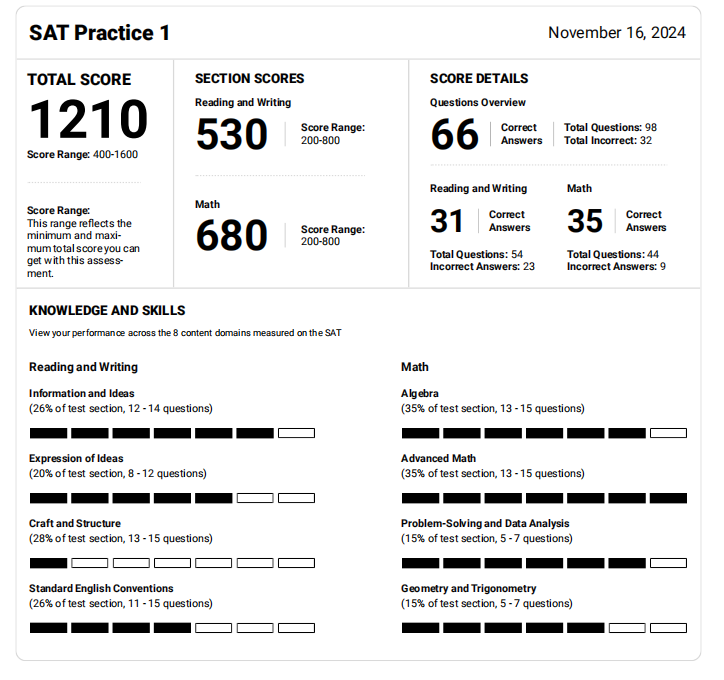
\includegraphics[width=1\linewidth]{E75.jpg}
\end{center}

\begin{center}
    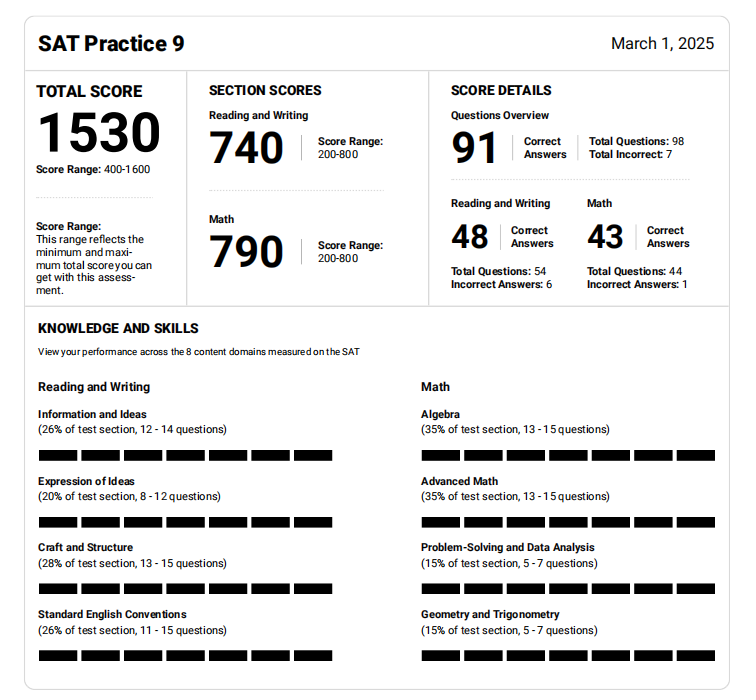
\includegraphics[width=1\linewidth]{E76.jpg}
\end{center}


\vspace{0.8cm}

\section*{\textcolor{RoyalBlue}{Test Schedule and Registration}}
\begin{definitionbox}{When and Where?}
The SAT is offered multiple times annually: \textbf{March, May, June, August, September, October, November, and December}. Test centers are available globally, including in mainland China, Hong Kong, and Macau.
\end{definitionbox}

\textbf{Registration:} Students can register through the \textit{official SAT website}.  
\textbf{Fees:} The standard registration fee is \textcolor{Red}{\$52}
\vspace{0.8cm}

\section*{\textcolor{RoyalBlue}{Scoring Requirements}}
\begin{tcolorbox}[colback=Lavender!5, colframe=RoyalBlue, title=\textbf{Scoring Benchmarks}]
\begin{itemize}
    \item \textcolor{ForestGreen}{\textbf{Maximum Score:}} \textcolor{Red}{1600 points}.
    \item \textcolor{ForestGreen}{\textbf{Top Universities:}} Often require \textcolor{Red}{1500+}.
    \item \textcolor{ForestGreen}{\textbf{Competitive Applicants:}} Scores above \textcolor{Red}{1300} are considered excellent.
    \item Students should set realistic goals based on their target schools.
\end{itemize}
\end{tcolorbox}

\vspace{0.8cm}

\section*{\textcolor{RoyalBlue}{Tips for Success}}
\begin{tcolorbox}[colback=Lavender!10, colframe=RoyalBlue, title=\textbf{Preparation Tips}]
\begin{itemize}
    \item \textbf{Practice Adaptive Testing:} Familiarize yourself with the adaptive format of the SAT.
    \item \textbf{Review Core Content:} Focus on algebra, geometry, critical reading, and analytical skills.
    \item \textbf{Time Management:} Practice under timed conditions to improve efficiency.
\end{itemize}
\end{tcolorbox}

\vspace{0.5cm}


\end{document}
